% !TEX TS-program = XeLaTeX
% !TEX encoding = UTF-8 Unicode

\chapter{基于相位比统计特征的脊柱姿态检测方法}
\label{chap03}
\defaultfont

\section{问题定义}
本文将脊柱姿态检测建模为基于 WiFi CSI 的文件级三分类问题。设一个原始 CSI 文件为 $X$，其对应的姿态标签集合为
\begin{equation}
\mathcal{Y}=\{y_1,y_2,y_3\},
\end{equation}
其中 $y_1$、$y_2$ 和 $y_3$ 分别表示正常姿态、脊柱后凸相关姿态和脊柱侧弯相关姿态。模型的目标是从 CSI 文件中提取能够反映人体姿态差异的特征，并学习特征向量到姿态类别之间的映射关系：
\begin{equation}
\hat{y}=f(X), \quad \hat{y}\in \mathcal{Y}.
\end{equation}

在无线感知场景中，人体位于发射端与接收端之间时，会对无线信号产生反射、遮挡、散射和多径传播等影响。不同脊柱姿态会改变人体躯干形态及其对无线传播路径的扰动方式，从而使 CSI 的相位比序列呈现出可区分的统计特征。本文利用这一特性进行非接触式脊柱姿态检测。

该问题建立在三个基本假设之上：采集阶段的类别标签能够反映预先定义的姿态状态；待检测数据与训练数据具有一致的 CSI 维度和链路排列；单个原始文件在其采集时段内主要对应一种姿态。若输入数据不满足这些条件，例如同时包含多种姿态转换或缺少必要天线链路，则固定长度文件级分类结果的含义需要重新评估。

\section{方法总体框架}
本文方法由 CSI 数据解析、接收天线相位比计算、相位展开、滑动窗口组织、文件级统计特征聚合、ExtraTrees 分类和检测结果输出组成。整体流程可表示为
\begin{equation}
X_{\mathrm{raw}}
\rightarrow X_{\mathrm{csi}}
\rightarrow X_{\mathrm{ratio}}
\rightarrow X_{\mathrm{stat}}
\rightarrow g(X_{\mathrm{stat}})
\rightarrow \hat{y},
\end{equation}
其中 $X_{\mathrm{raw}}$ 表示原始采集文件，$X_{\mathrm{csi}}$ 表示解析后的复数 CSI 数据，$X_{\mathrm{ratio}}$ 表示相位比序列，$X_{\mathrm{stat}}$ 表示文件级统计特征，$g(\cdot)$ 表示 ExtraTrees 分类器，$\hat{y}$ 表示最终输出的脊柱姿态类别。

系统首先从原始 \texttt{.dat} 文件中解析复数 CSI，获得时间帧、子载波、接收天线和发射天线维度上的信道响应；然后以第 0 根接收天线为参考，计算其他接收天线与参考天线之间的复数比值，并取幅角得到相位比；随后沿时间维度进行相位展开，减少相位周期跳变带来的不连续；最后将整个文件聚合为 1620 维统计特征，并输入 ExtraTrees 分类器进行三分类预测。

\section{文件级特征构建}
本文不直接将单个窗口作为最终分类对象，而是将一个原始 CSI 文件作为一次检测样本。这样做的原因是，脊柱姿态属于相对稳定的身体状态，单个短窗口可能只包含局部扰动，而完整文件能够更充分地保留一段采集过程中的整体统计规律。

对每个原始文件，系统首先生成长度为 512、步长为 256 的滑动窗口。每个窗口继承其所属文件的姿态标签，但窗口仅用于组织和统计特征，不作为最终投票单位。随后，系统汇总该文件全部窗口中的相位比序列，并对每一维相位比特征计算以下统计量：
\begin{enumerate}
\item 均值，用于描述相位比的整体水平；
\item 标准差，用于描述相位比的波动程度；
\item 10\% 分位数、中位数和 90\% 分位数，用于描述相位比分布；
\item 相邻帧差分绝对值均值，用于描述时间变化强度；
\item 相邻帧差分标准差，用于描述变化过程的稳定性；
\item 相位正弦均值和余弦均值，用于保留相位的周期性信息。
\end{enumerate}

由于每一时间帧具有 180 个相位比特征，每个特征对应 9 个统计量，因此每个 CSI 文件被表示为 1620 维文件级特征向量。该向量既包含整段采集数据的总体分布，也包含局部时间变化信息，能够作为传统机器学习分类器的输入。

\section{文件级建模与数据隔离}
本文选择文件级建模的另一个重要原因是控制数据相关性。采用重叠滑动窗口时，相邻窗口共享大量时间帧。如果将窗口随机划分到训练集、验证集和测试集，同一原始序列中的近似片段可能出现在不同子集中，使模型间接接触测试信息。即使最终指标较高，也难以判断模型学习到的是姿态规律还是原始序列的局部特征。

因此，完整流程应首先以原始文件或更高层级的独立采集单元划分数据，再分别执行窗口化和统计聚合。训练集用于学习模型参数，验证集用于比较模型和选择配置，测试集只用于最终评价。若研究目标是评价对陌生人员的泛化能力，还应进一步以受试者为分组单位进行划分，保证同一受试者的数据不会跨越训练集和测试集。

\section{ExtraTrees 分类模型}
ExtraTrees 即极端随机树集成模型，是一种由多棵随机决策树组成的监督分类方法。与普通决策树相比，ExtraTrees 在训练每棵树时引入更强的随机性：模型不仅随机选择候选特征，还随机生成候选切分阈值，再从中选择划分效果较好的节点切分方式。多棵树分别给出分类结果后，集成模型通过投票或概率平均输出最终类别。

设文件级统计特征为 $x\in \mathbb{R}^{1620}$，第 $m$ 棵树的预测结果为 $h_m(x)$，则由 $M$ 棵树组成的 ExtraTrees 分类器可表示为
\begin{equation}
g(x)=\operatorname{mode}\{h_1(x),h_2(x),\ldots,h_M(x)\}.
\end{equation}
本文最终模型使用 $M=700$ 棵极端随机树，并采用类别平衡权重、平方根特征采样和固定随机种子。类别平衡权重用于减小类别样本数量差异带来的影响；平方根特征采样使每棵树在不同特征子空间上学习分类规则；固定随机种子保证实验结果可复现。

ExtraTrees 适合本文任务的主要原因在于：首先，当前数据集文件数量有限，而统计特征维度较高，树集成模型能够在小样本高维特征上获得稳定表现；其次，树模型不依赖严格的特征缩放，对不同量纲的统计特征具有较好兼容性；最后，多棵树的集成能够表达复杂的非线性特征组合，适合处理多天线、多子载波 CSI 特征之间的交互关系。

\section{训练与分类决策机制}
模型训练阶段仅使用训练集中的文件级特征估计树节点的划分规则。验证集用于比较候选模型、树数量、特征采样方式和类别权重等配置。模型配置确定后，测试集保持封闭，直至最终性能评价。该顺序能够减少反复查看测试结果造成的选择偏差，使测试指标更接近一次独立评价。

对于单个待检测文件，每棵树根据其学习到的节点规则给出类别判断，集成模型再通过投票或类别概率平均形成最终结果。如果应用场景需要表达不确定性，可以同时保留各类别的投票比例或预测概率，并设置低置信度拒绝机制。拒绝机制不改变分类模型本身，而是在证据不足时避免输出过于确定的类别。由于本文实验主要评价三分类性能，最终结果仍以离散类别和分类指标为主。

为分析最终模型实际使用的信息，本文进一步统计 700 棵树基于不纯度下降得到的特征重要性，并分别按统计量类型聚合及列出重要性最高的具体特征，如图~\ref{fig:extratrees_importance} 所示。正弦均值与余弦均值的累计贡献最高，二者合计约占总重要性的 40\%，说明保留相位周期结构对分类具有明显作用；差分绝对值均值与差分标准差也占有较高权重，表明时间变化强度是姿态区分的重要依据。排名靠前的具体特征主要集中在若干子载波的 RX2/RX1 相位比链路。需要指出的是，该重要性反映模型内部的相对分裂贡献，不表示特征与姿态之间存在直接因果关系。

\begin{figure}[htbp]
\centering
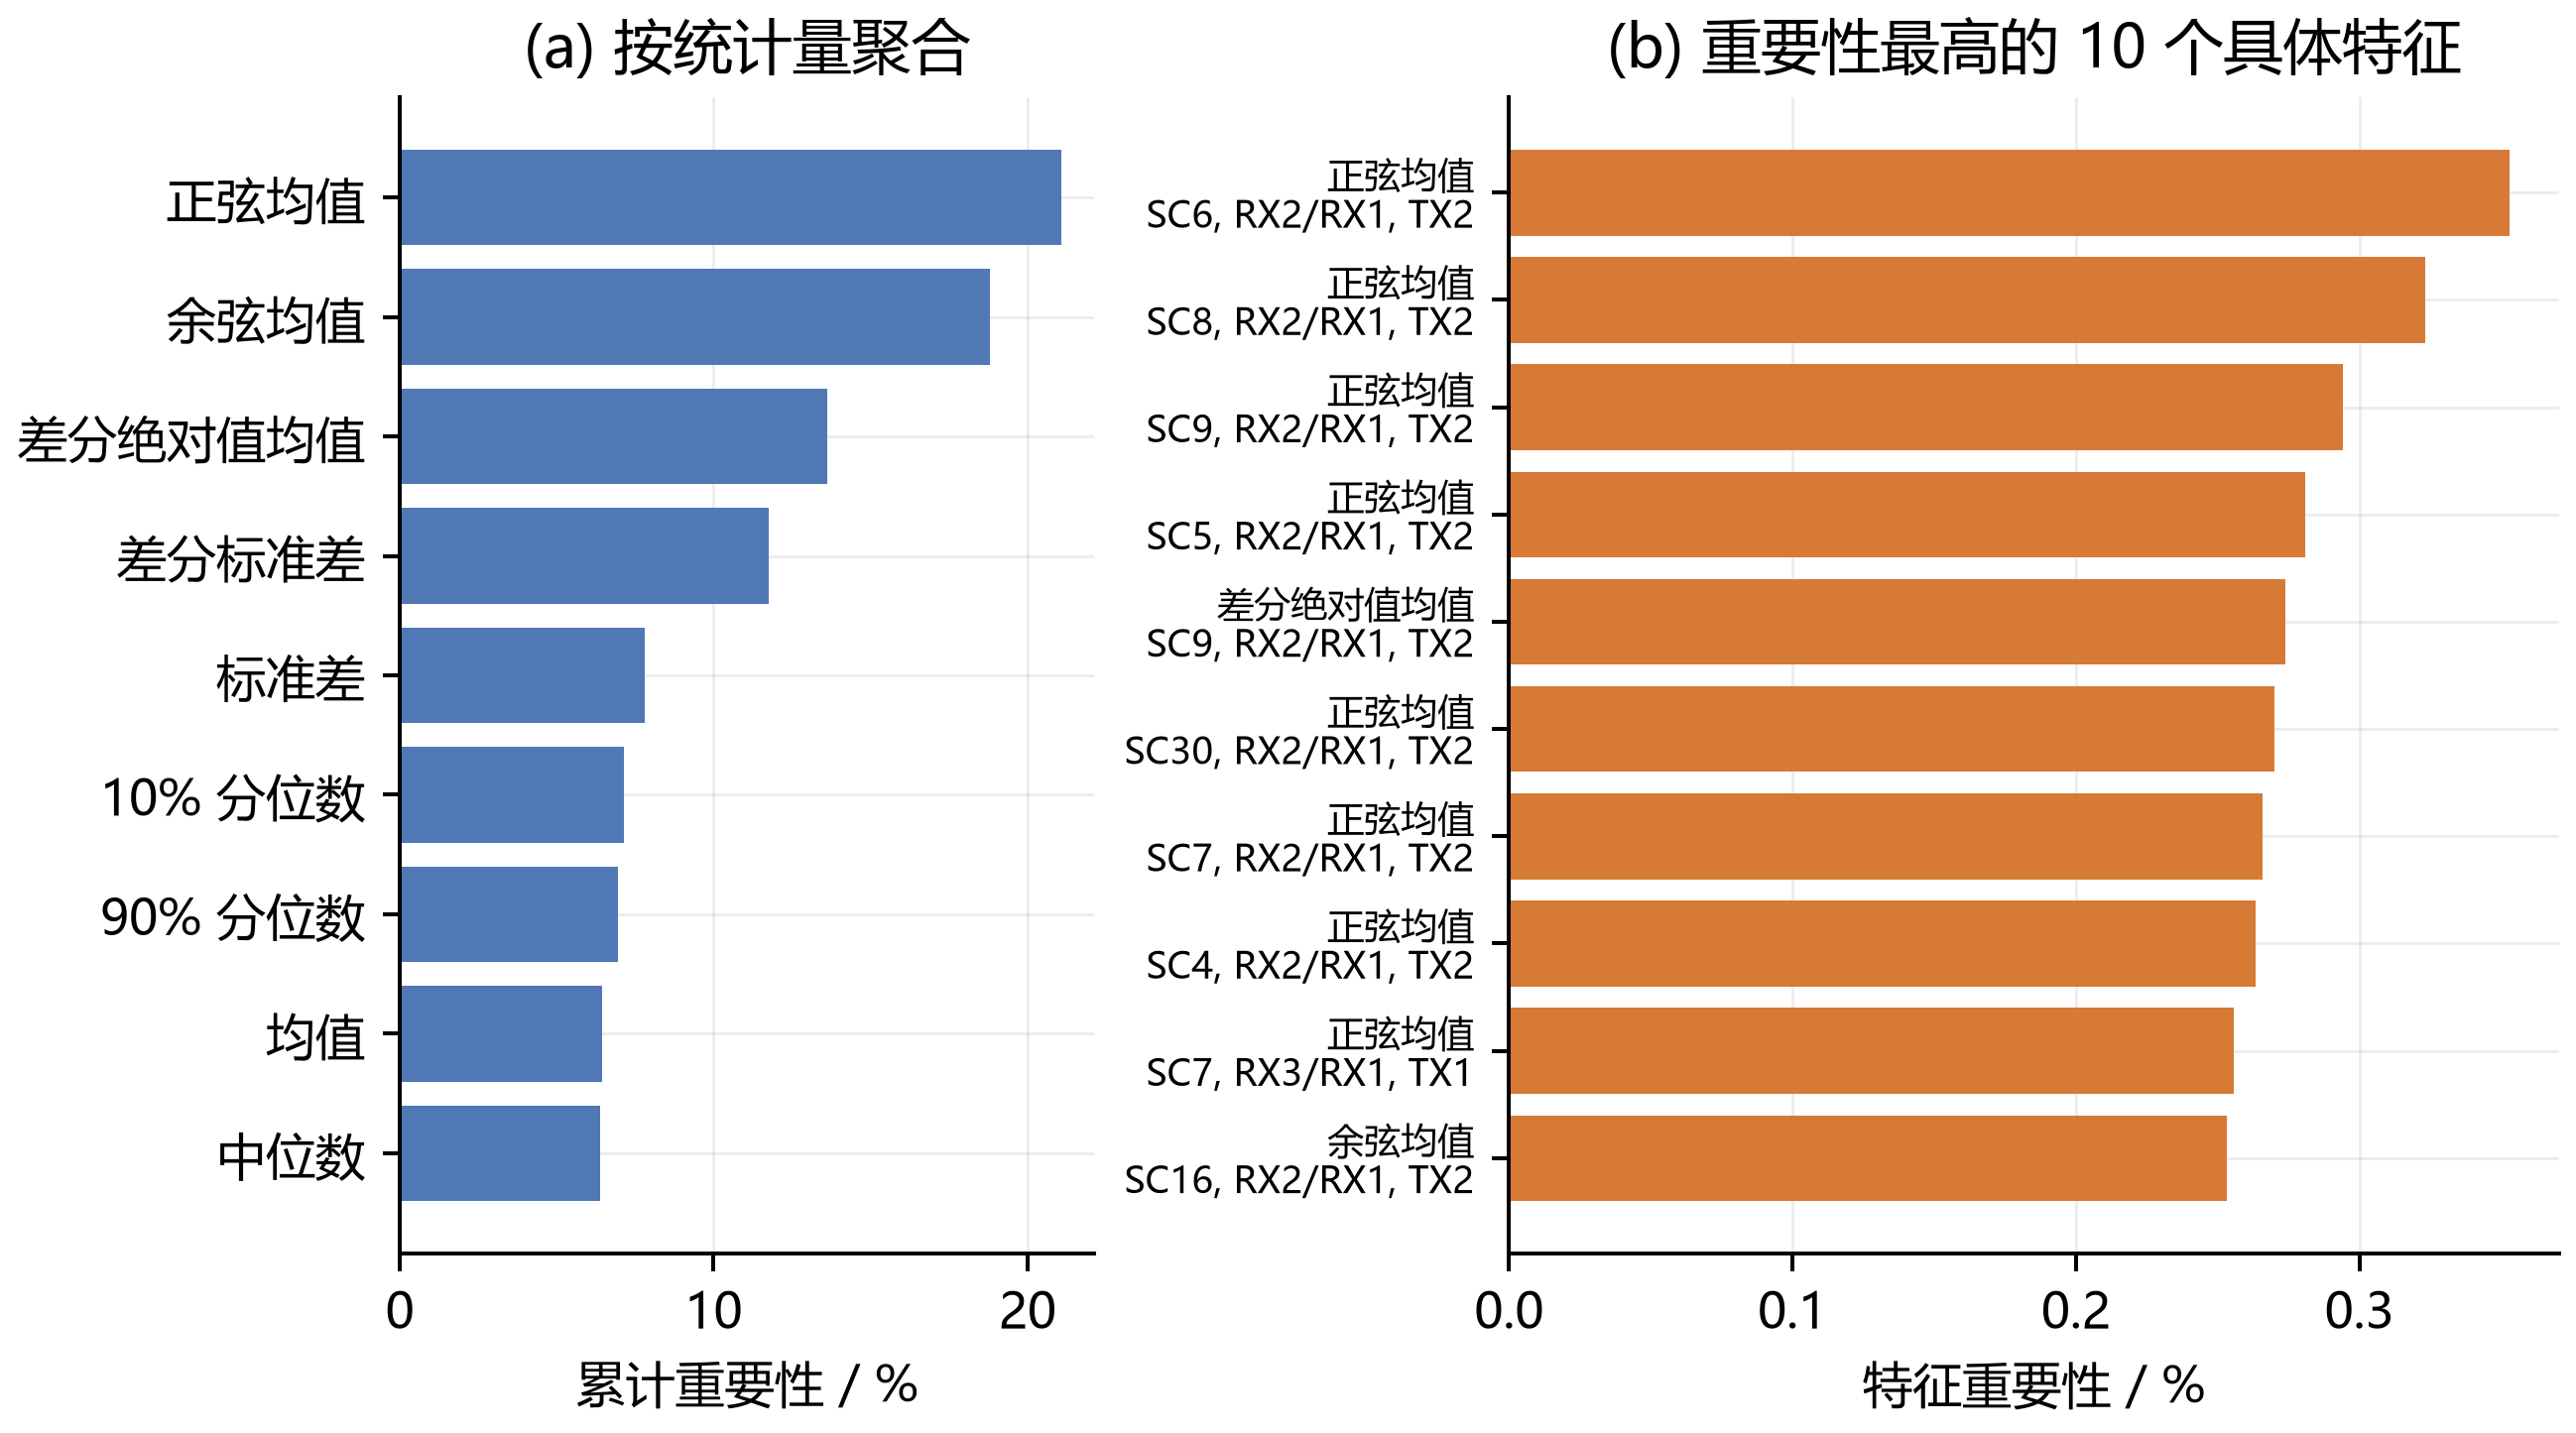
\includegraphics[width=0.96\textwidth]{figures/extratrees_feature_importance.png}
\caption{ExtraTrees 模型的特征重要性分析}
\label{fig:extratrees_importance}
\end{figure}

\section{检测结果输出}
检测阶段对待检测 CSI 文件执行与训练阶段相同的数据处理流程。系统解析复数 CSI，计算接收天线相位比并进行时间相位展开，随后生成滑动窗口并聚合为 1620 维文件级统计特征。训练完成的 ExtraTrees 模型根据该特征向量输出三类姿态的预测结果。

该流程实现了从 WiFi CSI 原始文件到脊柱姿态类别的完整检测。由于检测过程不依赖摄像头图像或可穿戴设备，系统具有非接触、低侵入和隐私友好的特点，适用于室内场景下的人体姿态感知与脊柱健康辅助检测研究。

\section{算法流程与复杂度分析}
从算法结构看，方法可以概括为数据解析、相对相位构造、时间组织、统计聚合和集成分类五个阶段。训练阶段在上述特征处理之后增加模型拟合和配置选择，检测阶段则加载已经确定的模型执行分类。两个阶段共享同一特征构建过程，从而避免训练与检测使用不同处理规则。

设单个文件包含 $T$ 个时间帧，每帧相位比维度为 $D$，统计量数量为 $K$。相位比计算、时间展开和统计聚合的主要计算量随 $T$ 和 $D$ 近似线性增长，生成的文件级向量维度为 $D K$。对于包含 $M$ 棵树的集成模型，单次分类需要沿每棵树的决策路径进行判断，其开销与树数量和平均树深相关。与直接对长序列执行多层神经网络相比，文件级统计表示能够在分类阶段降低输入规模，但代价是压缩部分精细时序信息。

该复杂度分析说明，方法适合以完整采集文件为单位进行批量训练和检测。若扩展到实时连续监测，需要进一步设计增量窗口更新、在线质量检查和连续结果平滑机制，而不能简单地将离线文件分类结果等同于实时输出。

\section{本章小结}
本章将脊柱姿态检测形式化为文件级监督分类问题，并给出了从原始 CSI 到类别输出的完整方法。通过先划分原始文件、再生成窗口，可以降低高度相关片段跨越数据子集造成的信息泄漏风险；通过文件级统计表示和 ExtraTrees 集成决策，可以在有限样本和高维特征条件下建立分类模型。最后，本章讨论了训练与检测的一致性、低置信度输出以及方法的计算复杂度，为后续实验设计提供依据。
